%%%%%%%%%%%%%%%%%%%%%%%%%%%%%%%%%%%%%%%%%%%%%%%%%
%         ARQUIVO LATEX - ARTIGO TCC
%%%%%%%%%%%%%%%%%%%%%%%%%%%%%%%%%%%%%%%%%%%%%%%%%
\documentclass[sigconf]{acmart}

% --- PACOTES ESSENCIAIS ---
\usepackage[utf8]{inputenc} % Permite acentuação em português
\usepackage{graphicx}       % Para incluir figuras
\usepackage{booktabs}       % Para tabelas com qualidade (top, mid, bottomrule)
\usepackage{amsmath}        % Para símbolos matemáticos como R^2
\usepackage{textcomp}       % Para símbolo de copyright, etc.
\usepackage{lipsum}         % Apenas para texto de exemplo (pode remover)

\renewcommand{\figurename}{Figura}
\renewcommand{\tablename}{Tabela}
\renewcommand{\keywordsname}{Palavras-chave}

%%%%%%%%%%%%%%%%%%%%%%%%%%%%%%%%%%%%%%%%%%%%%%%%%
%         BLOCO DE COPYRIGHT - SBC
%%%%%%%%%%%%%%%%%%%%%%%%%%%%%%%%%%%%%%%%%%%%%%%%%
\setcopyright{none}
\acmConference[COTB '25]{Computer on the Beach '25}{Abril 01--03, 2025}{Florianópolis, SC}
\acmBooktitle{Anais do Computer on the Beach 2025 (COTB '25), Abril 01--03, 2025, Florianópolis, SC}
\acmPrice{}
\acmISBN{}
\acmDOI{} 

% --- METADADOS DO ARTIGO ---
\title{Predição de Peso da Tilápia do Nilo por Meio do Fenótipo Usando Redes Neurais Convolucionais}

\author{Henrique Yoshiharu Kajihara}
\affiliation{
  \institution{Universidade Estadual de Maringá (UEM)}
  \streetaddress{Av. Colombo, 5790 - Bloco C56}
  \city{Maringá}
  \state{Paraná}
  \country{Brasil}
  \postcode{87020-900}
}
\email{henriqueykajihara@gmail.com} 

\author{Josiane Melchiori Pinheiro}
\affiliation{
  \institution{Universidade Estadual de Maringá (UEM)}
  \city{Maringá}
  \state{Paraná}
  \country{Brasil}
}
\email{jmpferreira@uem.br}

% --- RESUMO / ABSTRACT ---
\begin{abstract}
Biometric analysis in fish farms, such as weighing and measuring Nile tilapia, is a manual and stressful procedure for the animals and incurs significant costs, leading to growth delays and stock losses. This study investigates the application of Convolutional Neural Networks (CNNs) to estimate tilapia weight from images of its phenotype, with the aim of automating and optimizing this process. Using an existing image dataset, several CNN models were trained and evaluated. The results are promising, with some configurations achieving discrepancies of only 45–50 grams between predicted and actual weight, and a coefficient of determination ($R^2$) of 0.97. It is concluded that it is feasible to develop an efficient and accurate system to predict the weight of Nile tilapia using CNNs, with potential to increase productivity and reduce costs in fish farming.
\end{abstract}

% --- CCS (ACM Computing Classification System) ---
% Ferramenta para gerar: https://dl.acm.org/ccs
\begin{CCSXML}
<ccs2012>
  <concept>
    <concept_id>10010147.10010257.10010293.10010294</concept_id>
    <concept_desc>Computing methodologies~Neural networks</concept_desc>
    <concept_significance>500</concept_significance>
  </concept>
  <concept>
    <concept_id>10010147.10010178.10010224.10010245.10010251</concept_id>
    <concept_desc>Computing methodologies~Object recognition</concept_desc>
    <concept_significance>300</concept_significance>
  </concept>
  <concept>
    <concept_id>10003752.10003809.10003716.10011136.10011137</concept_id>
    <concept_desc>Applied computing~Agriculture</concept_desc>
    <concept_significance>400</concept_significance>
  </concept>
</ccs2012>
\end{CCSXML}

\ccsdesc[500]{Computing methodologies~Neural networks}
\ccsdesc[300]{Computing methodologies~Object recognition}
\ccsdesc[400]{Applied computing~Agriculture}

% --- PALAVRAS-CHAVE ---
\keywords{Inteligência Artificial (IA), Redes Neurais Convolucionais (CNNs), Visão Computacional, Tilápia do Nilo, Piscicultura, Predição de Peso.}

% --- INÍCIO ---
\begin{document}

\maketitle

% --------------------------------------------------------------
\section{Introdução}
% --------------------------------------------------------------
A tecnologia tem se tornado fundamental no agronegócio para otimização de custos e lucros. Na piscicultura da Tilápia do Nilo, a análise biométrica é crucial para acompanhar a evolução do cardume. Este manejo, no entanto, é quase inteiramente manual, exigindo a retirada dos peixes da água para medição e pesagem.

Esse processo é altamente estressante para os animais \cite{Iwama1997}, causando alterações fisiológicas que levam à baixa imunidade, diminuição da taxa de crescimento e, em alguns casos, mortalidade \cite{Iwama1997, Barcellos2000}. Além de custoso e demorado, o método invasivo impacta diretamente o bem-estar animal e a produtividade. Segundo a Associação Brasileira de Psicultura, a tilápia representa aproximadamente 65\% da produção de peixes de cultivo no Brasil, que é o quarto maior produtor mundial dessa espécie \cite{PeixeBR2023}. Entre 2014 e 2023, a produção aquícola nacional saltou de 578{,}8 mil para 887{,}0 mil toneladas, um aumento superior a 50\%, o que torna ainda mais urgente a modernização das etapas de monitoramento zootécnico \cite{PeixeBR2023}.

Do ponto de vista fisiológico, o estresse desencadeado pelo manejo é descrito em três níveis: efeitos primários, relacionados ao aumento de hormônios como catecolaminas e corticosteróides; efeitos secundários, que incluem alterações metabólicas em parâmetros como glicemia, glicogênio e ácido lático; e efeitos terciários, expressos em queda de desempenho produtivo, reprodutivo e maior susceptibilidade a doenças \cite{Iwama1997, Barcellos2000}. Em conjunto, esses efeitos reforçam que a minimização da manipulação física dos peixes não é apenas uma questão de conforto animal, mas também de eficiência produtiva.

Neste contexto, as Redes Neurais Convolucionais (CNNs) surgem como uma alternativa promissora. Este estudo propõe a aplicação de técnicas de \textit{Deep Learning} para estimar o peso de tilápias de forma automatizada e não intrusiva, a partir de imagens. O objetivo geral é reduzir o tempo de manejo e o estresse animal, implementando um algoritmo que realize a predição de peso de maneira rápida e eficaz. As imagens utilizadas foram cedidas por um estudo anterior focado em rendimento de carcaça \cite{Cardoso2021}.

Além do impacto direto na rotina de manejo, a automação da biometria pode contribuir com um uso mais racional de insumos, especialmente ração, ao permitir o ajuste fino de planos alimentares com base em estimativas de peso mais frequentes e menos dependentes de intervenção humana. Em um cenário de margens estreitas e alta competitividade, pequenas melhorias na eficiência de conversão alimentar podem representar ganhos financeiros significativos ao longo de um ciclo produtivo completo.

A relevância da abordagem proposta também está alinhada com demandas contemporâneas por sistemas produtivos mais éticos e sustentáveis. Métodos de biometria menos invasivos favorecem o bem-estar animal e podem apoiar processos de certificação, agregando valor ao produto final. Ao mesmo tempo, o uso de visão computacional e IA aproxima a piscicultura de conceitos de agricultura 4.0, abrindo espaço para integrações futuras com sensores, sistemas embarcados e plataformas de monitoramento em tempo real.

Dessa forma, este trabalho se insere na interseção entre Inteligência Artificial, visão computacional e produção animal, investigando a viabilidade de um modelo de CNN para predição de peso de Tilápia do Nilo a partir de imagens obtidas em ambiente experimental, mas com características próximas da realidade de campo.

% --------------------------------------------------------------
\section{Trabalhos Relacionados}
% --------------------------------------------------------------
A aplicação de visão computacional para estimar características fenotípicas não é nova, mas sua aplicação em piscicultura é menos explorada.

Ma et al. \cite{Ma2024} revisaram mais de 70 pesquisas sobre o uso de aprendizado de máquina (incluindo regressão linear e redes neurais) em imagens 2D e 3D para estimar o peso de suínos e bovinos. Eles destacam que a abordagem reduz o estresse animal e permite a coleta massiva de dados, alcançando erros percentuais tão baixos quanto 4,87\% em alguns casos. No entanto, apontam desafios como a necessidade dos animais permanecerem parados para imagens 3D e o alto custo de sensores de boa qualidade.

Lee, Lee e Cho \cite{Lee2023} utilizaram redes neurais profundas em imagens 2D para estimar o peso de bovinos. O estudo comparou métodos de segmentação, utilizando Mask R-CNN (segmentação totalmente supervisionada) e alcançando uma margem de erro de 5,06\% em um conjunto de 43 animais.

Inspirado por esses avanços, este trabalho aplica técnicas similares de redes neurais profundas ao estudo de tilápias, adaptando as estratégias para os desafios específicos da piscicultura.

Apesar dos resultados promissores em suínos e bovinos, observa-se uma lacuna quando se trata de espécies aquáticas. A maior parte dos trabalhos ainda se concentra em ambientes controlados, com câmeras e sensores dedicados, o que dificulta a transferência direta dessas soluções para a realidade de sistemas aquícolas de baixo custo. Além disso, contribuições como a de Cardoso et al. \cite{Cardoso2021} exploram análise de imagens para estimativa de rendimento de carcaça, mas não abordam explicitamente a predição de peso a partir de CNNs. Assim, o presente estudo contribui ao explorar um cenário intermediário, em que se utilizam imagens coletadas em ambiente experimental realista, com iluminação e posicionamento não totalmente padronizados, aproximando-se das condições encontradas por produtores.

% --------------------------------------------------------------
\section{Metodologia}
% --------------------------------------------------------------
O desenvolvimento foi conduzido em etapas sistemáticas, desde a aquisição dos dados até a avaliação do modelo.

\subsection{Materiais e Ambiente}
\textbf{Banco de Imagens:} Foram utilizadas 5975 imagens no formato JPG de 1195 tilápias (5 imagens de cada animal em ângulos diversos). Os dados foram obtidos na base experimental da PEIXEGEN/UEM, provenientes do estudo de Cardoso et al. \cite{Cardoso2021} e possuem aprovação da Comissão de Ética no Uso de Animais (CEUA/UEM). As imagens originais foram capturadas com fundo azul uniforme e uma régua de 30 cm imediatamente abaixo dos peixes, permitindo a utilização da escala como referência de tamanho. O estudo de origem empregou imagens RGB e em profundidade para estimar rendimento de filé \cite{Cardoso2021}, porém, neste trabalho foram utilizadas apenas as imagens RGB.

A Figura~\ref{fig:coleta} ilustra o processo de coleta das tilápias para registro das imagens, em ambiente de campo, enquanto a Figura~\ref{fig:exemplar_tilapia} apresenta um exemplo de imagem bruta utilizada como entrada da CNN, evidenciando o padrão de fundo e referência de escala adotados.

\begin{figure}[h]
\centering
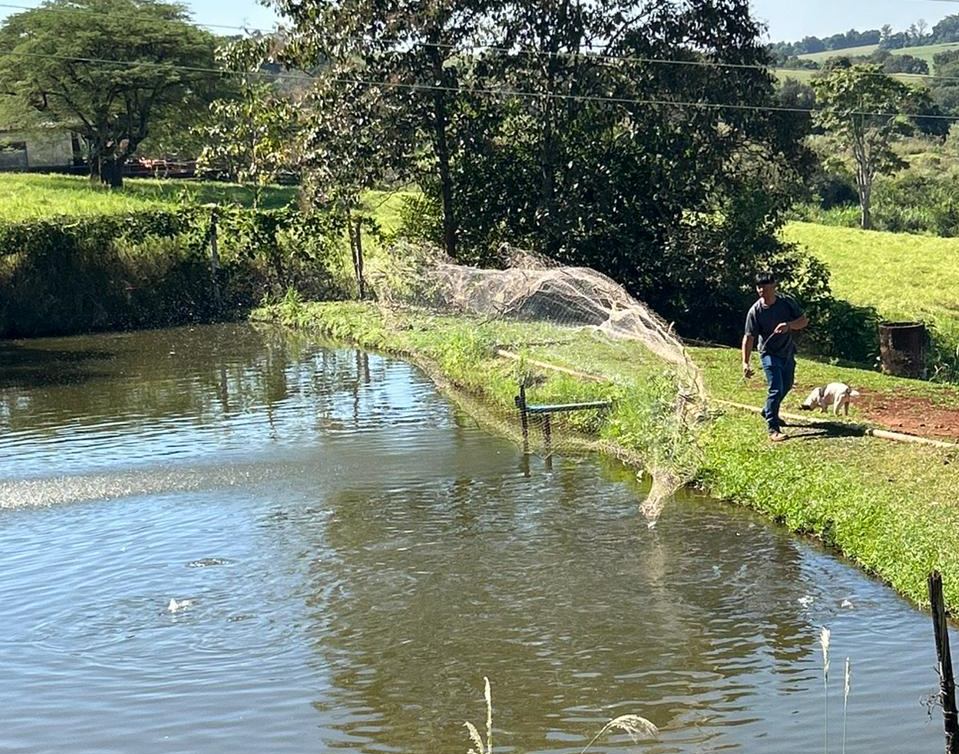
\includegraphics[width=\linewidth]{figura1.png}
\caption{Processo de captura das imagens no ambiente experimental, com uso de tarrafa para coleta seletiva das tilápias.}
\label{fig:coleta}
\Description{Zootecnista utilizando uma tarrafa para coletar tilápias em tanque ou viveiro, representando o procedimento de captura dos animais para registro das imagens.}
\end{figure}

\begin{figure}[h]
\centering
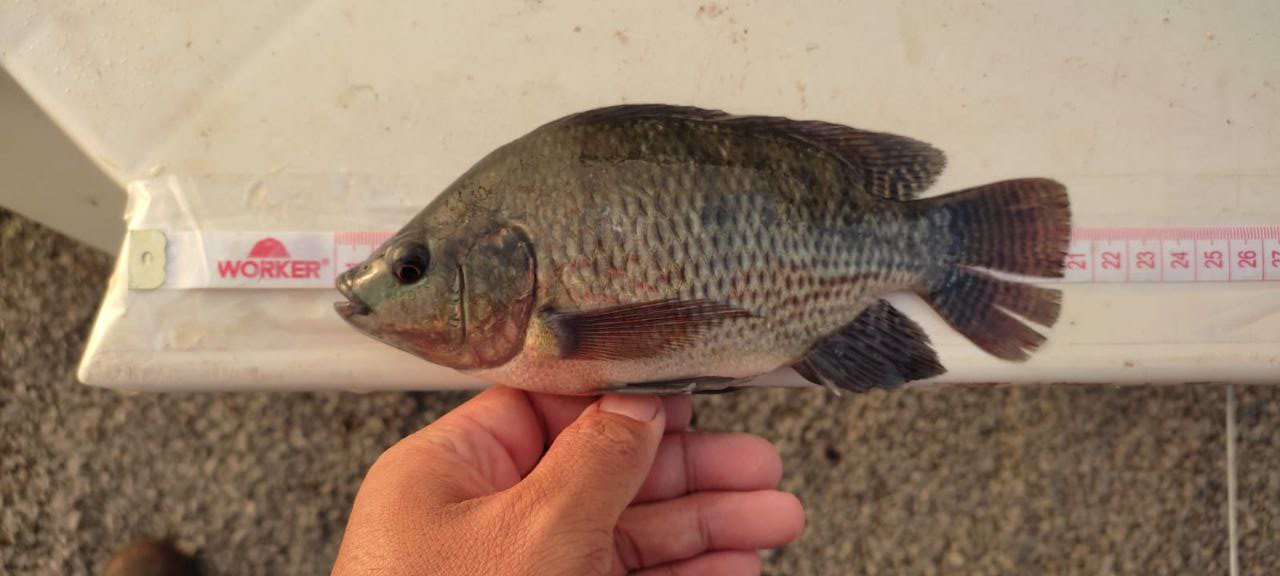
\includegraphics[width=0.37\textheight]{figura2.png}
\caption{Exemplo de imagem bruta de Tilápia do Nilo utilizada como entrada da CNN.}
\label{fig:exemplar_tilapia}
\Description{Tilápia posicionada sobre um fundo azul com uma régua de 30 cm logo abaixo, representando o padrão de captura das imagens usadas no experimento.}
\end{figure}

\textbf{Ferramentas:} O modelo foi implementado em Python 3.12, utilizando TensorFlow 2.18.0, OpenCV, Pandas e Matplotlib. Essas bibliotecas foram escolhidas por oferecerem suporte consolidado à construção de redes neurais profundas, processamento de imagens e visualização de resultados.

\textbf{Ambiente Experimental:} Os experimentos foram executados em um computador com processador Intel Core i7-12650H e 32 GB de RAM DDR4. Não foi utilizada GPU dedicada, o que motivou a adoção de uma arquitetura de CNN de complexidade moderada, visando equilibrar desempenho e custo computacional.

\textbf{Análise exploratória das imagens:} Antes do treinamento, foi realizada uma inspeção visual das imagens e dos metadados associados, com o objetivo de identificar padrões de iluminação, variações de enquadramento e presença de reflexos. Observou-se que, embora o cenário de captura fosse controlado (fundo azul e régua fixa), havia variações relevantes na posição dos peixes em relação à câmera e na incidência de luz, fatores que impactaram diretamente a qualidade do pré-processamento e a estabilidade do treinamento.

\textbf{Preparação dos rótulos:} Os pesos das tilápias variavam em uma faixa aproximada entre 400 g e 2000 g. Para facilitar o treinamento e reduzir a sensibilidade a diferenças de escala, os valores foram normalizados por meio de uma transformação do tipo \textit{min-max}. Essa normalização contribuiu para gradientes mais estáveis nas primeiras épocas, facilitando a convergência dos otimizadores Adam e Nadam.

\textbf{Divisão dos conjuntos de dados:} A divisão entre treino e teste foi realizada de forma a garantir que um mesmo indivíduo (peixe) não aparecesse simultaneamente em ambos os conjuntos. Dessa forma, cada peixe contribuiu com todas as suas imagens para apenas uma partição, reduzindo o risco de vazamento de informação. O conjunto de treinamento foi composto por 1000 peixes (5000 imagens) e o conjunto de teste por 195 peixes (975 imagens), preservando a diversidade de pesos em ambas as partições.

\subsection{Arquitetura do Modelo Proposto}
Foi desenvolvida uma CNN para regressão, projetada para processar imagens de entrada de $128 \times 128 \times 3$ pixels (RGB). A arquitetura, resumida na Tabela \ref{tab:arquitetura}, foi baseada em estudos de visão computacional para tarefas similares.

\begin{table}[h]
\caption{Resumo da arquitetura da CNN proposta.}
\label{tab:arquitetura}
\centering
\begin{tabular}{@{}lll@{}}
\toprule
\textbf{Camada} & \textbf{Configuração} & \textbf{Função de Ativação} \\
\midrule
Entrada          & Imagem $128 \times 128 \times 3$ &             \\
\midrule
Convolucional 1  & 32 filtros $3 \times 3$          & ReLU        \\
MaxPooling 1     & $2 \times 2$                     & -           \\
\midrule
Convolucional 2  & 64 filtros $3 \times 3$          & ReLU        \\
MaxPooling 2     & $2 \times 2$                     & -           \\
\midrule
Convolucional 3  & 128 filtros $3 \times 3$         & ReLU        \\
MaxPooling 3     & $2 \times 2$                     & -           \\
\midrule
Convolucional 4  & 256 filtros $3 \times 3$         & ReLU        \\
MaxPooling 4     & $2 \times 2$                     & -           \\
\midrule
Flatten          & -                                & -           \\
\midrule
Dense 1          & 512 neurônios                    & ReLU        \\
Dropout          & Taxa 0.5                         & -           \\
\midrule
Dense 2          & 256 neurônios                    & ReLU        \\
Dropout          & Taxa 0.5                         & -           \\
\midrule
Dense 3          & 128 neurônios                    & ReLU        \\
\midrule
Saída (Regressão)& 1 neurônio                      & Linear      \\
\bottomrule
\end{tabular}
\end{table}

As camadas convolucionais extraem características visuais, enquanto as camadas de \textit{pooling} reduzem a dimensionalidade espacial. Regularização L2 foi aplicada às camadas densas e \textit{Dropout} foi usado para mitigar \textit{overfitting}. A opção por uma arquitetura relativamente compacta também se justifica pela ausência de GPU no ambiente experimental, tornando inviável, neste momento, o uso de modelos significativamente mais profundos, como ResNets ou EfficientNets \cite{Goodfellow2016}.

\subsection{Treinamento e Execução}
\textbf{Função de Perda e Otimização:} Utilizou-se o Erro Absoluto Médio (MAE) como função de perda, por ser diretamente interpretável em termos de gramas de diferença entre o peso real e o predito. Foram testados comparativamente os otimizadores \textbf{Adam} e \textbf{Nadam}.

\textbf{Scheduler de taxa de aprendizado:} Foi adotada uma estratégia de redução dinâmica da taxa de aprendizado, de forma que, após determinado número de épocas sem melhora na métrica de validação, a taxa fosse reduzida em um fator de 0,1, permitindo um refinamento mais preciso dos pesos nas etapas finais de treinamento.

\textbf{Aumento de Dados (Data Augmentation):} Devido ao banco de dados limitado, um \texttt{ImageDataGenerator} foi usado para criar variações artificiais das imagens (rotação, zoom, \textit{flip}), ampliando dinamicamente o conjunto de treino. Em termos práticos, isso significa que, em um treinamento com 20 épocas, o modelo pôde ser exposto, de forma virtual, a um número de amostras muito superior ao número de imagens originalmente rotuladas.

\textbf{Conjunto de Dados:} O modelo foi treinado com 5.000 imagens (1.000 peixes) e avaliado em um conjunto de teste independente de 975 imagens (195 peixes).

\textbf{Experimentos:} Foram realizados quatro experimentos principais, variando o otimizador (Adam/Nadam) e o uso (ou não) de um \textit{pipeline} de pré-processamento de imagens com OpenCV. Em todos os casos, o estado interno dos modelos era reinicializado entre execuções, garantindo independência entre experimentos e maior confiabilidade na comparação das configurações.

% --------------------------------------------------------------
\section{Resultados e Discussão}
% --------------------------------------------------------------
As métricas de avaliação primárias foram o \textbf{Erro Absoluto Médio (MAE)} e o \textbf{Coeficiente de Determinação ($R^2$)}.

\subsection{Falha no Pré-processamento}
Uma descoberta inicial significativa foi que o \textit{pipeline} de pré-processamento desenvolvido com OpenCV (incluindo ajuste de brilho, conversão HSV e aplicação de máscaras) não foi satisfatório.

Como visto na Figura \ref{fig:preprocessamento}, o processo falhou em segmentar corretamente o peixe em muitas imagens, removendo informações essenciais (partes do peixe) ou falhando em remover o fundo. Isso foi atribuído à variabilidade de iluminação e reflexos nas imagens originais. Consequentemente, os modelos treinados com imagens pré-processadas tiveram desempenho drasticamente inferior, indicando que a CNN ``crua'' foi mais eficaz em lidar com os dados originais.

\begin{figure}[h]
\centering
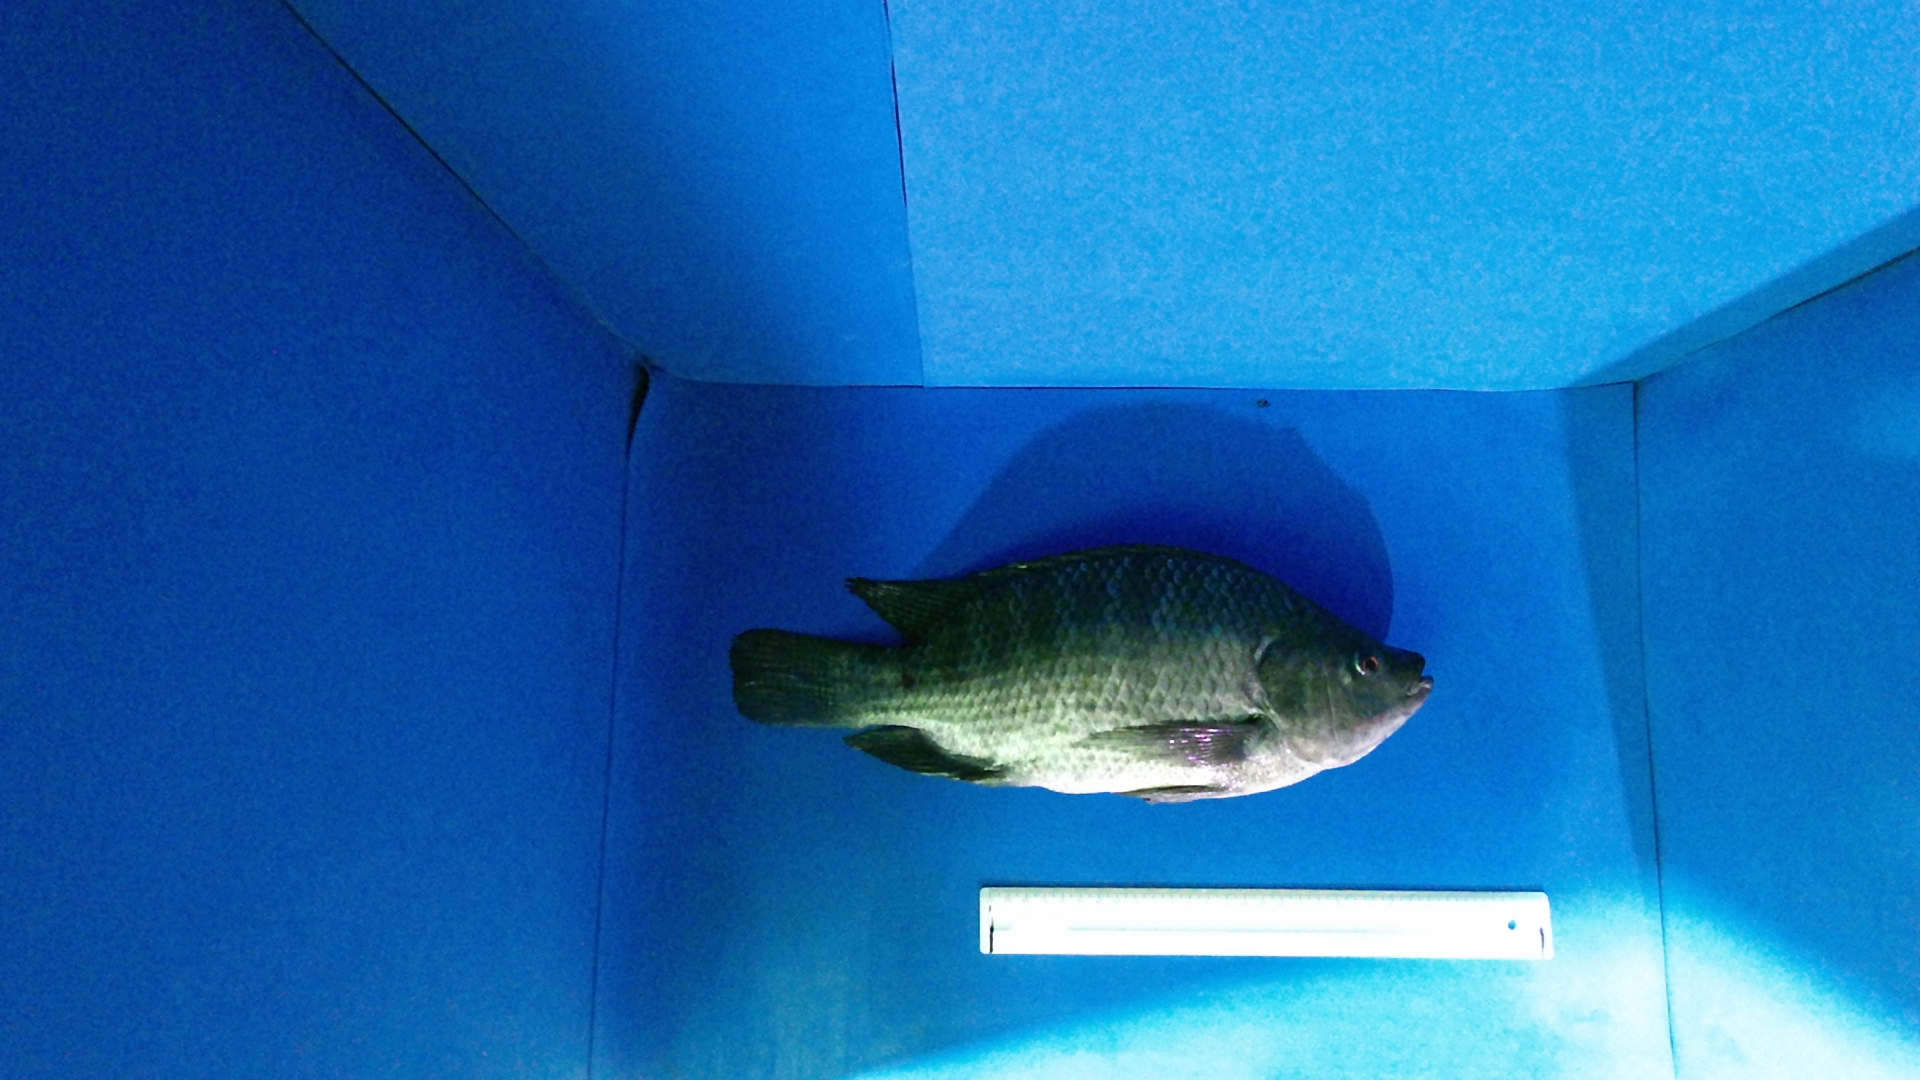
\includegraphics[width=0.48\linewidth]{figura12.jpg}
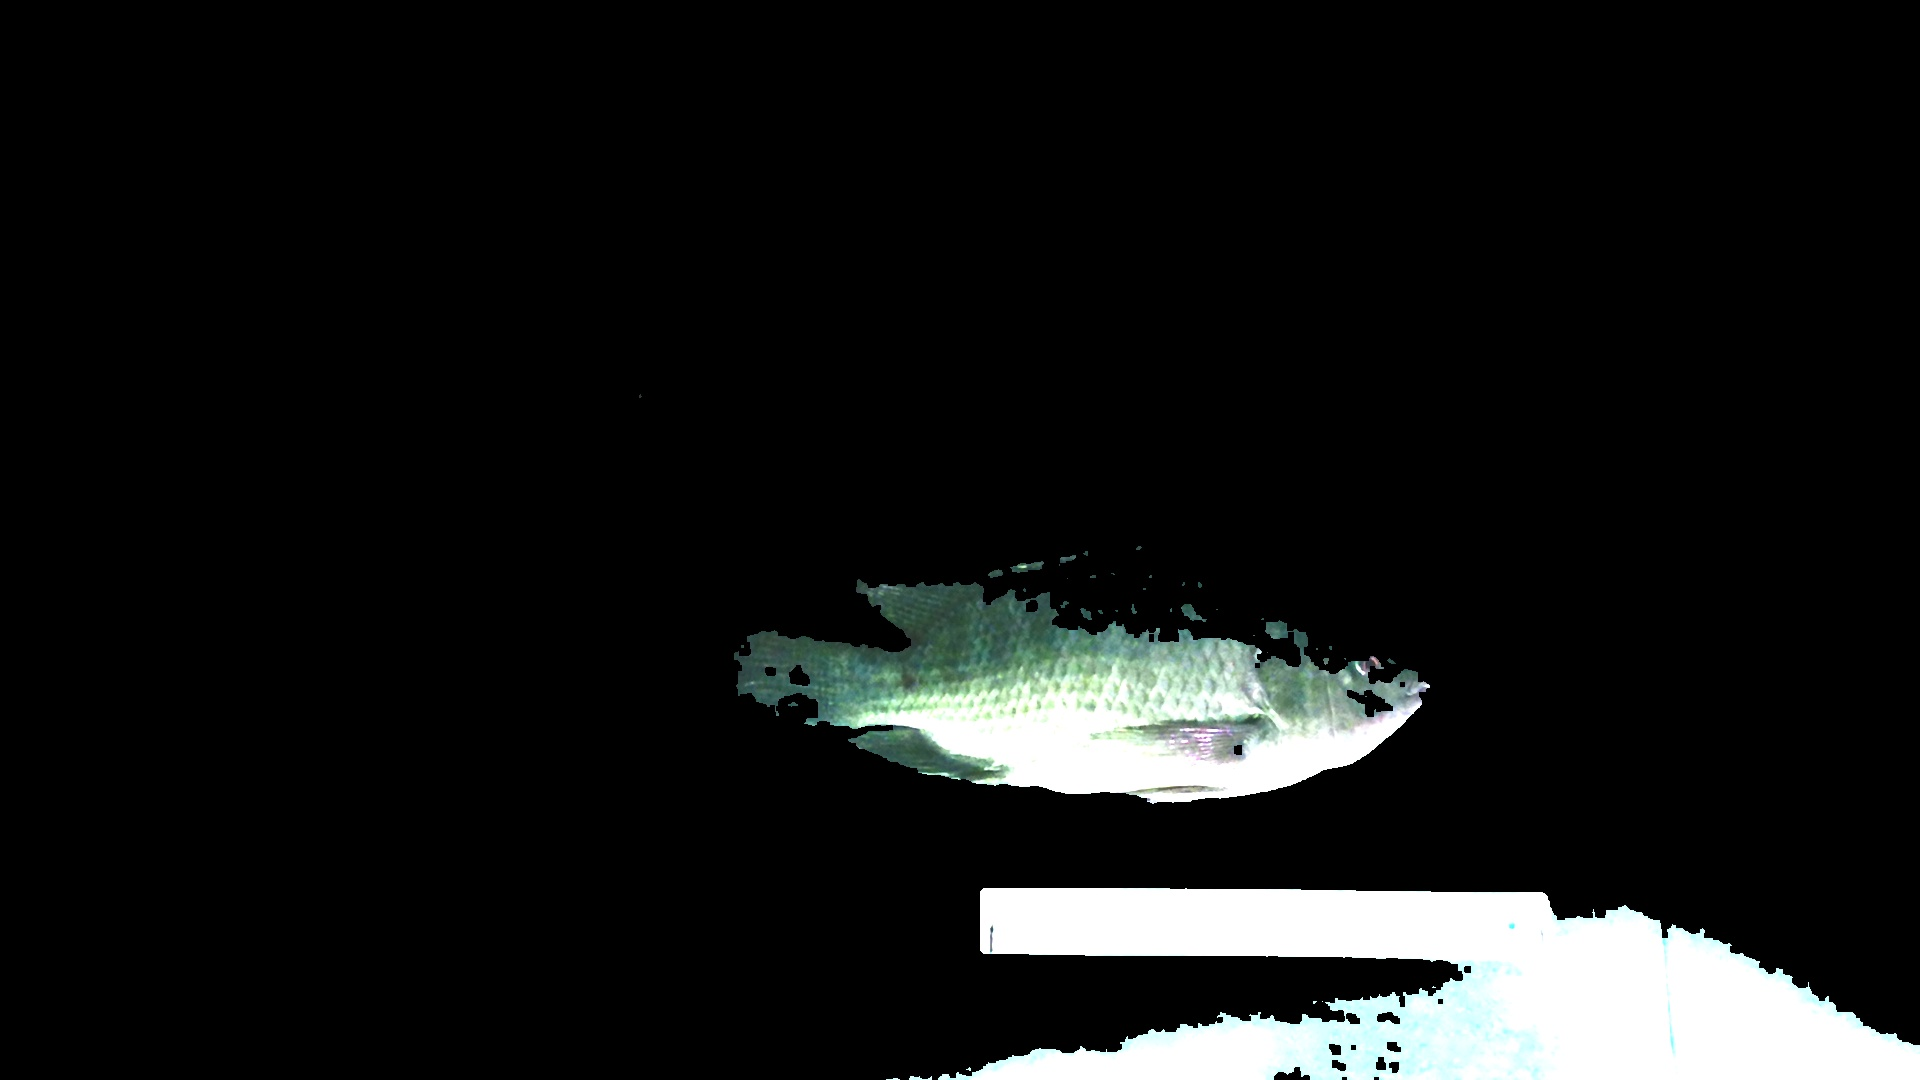
\includegraphics[width=0.48\linewidth]{figura13.jpg}
\caption{Comparação da imagem original (esquerda) e o resultado do pré-processamento com falha (direita), que removeu partes do peixe.}
\label{fig:preprocessamento}
\Description{Duas imagens de uma tilápia. A da esquerda mostra o peixe inteiro contra um fundo azul. A da direita mostra o resultado de um pré-processamento ruim, onde o fundo está preto, mas partes do peixe também foram apagadas.}
\end{figure}

\subsection{Resultados dos Modelos}
Os melhores resultados foram consistentemente obtidos sem o pré-processamento. A Tabela \ref{tab:resultados_comparativos} sumariza os melhores desempenhos encontrados para os otimizadores Adam e Nadam (sem pré-processamento).

\begin{table}[h]
\caption{Melhores resultados obtidos (sem pré-processamento).}
\label{tab:resultados_comparativos}
\centering
\begin{tabular}{@{}lcccc@{}}
\toprule
\textbf{Otimizador} & \textbf{Épocas} & \textbf{Semente} & \textbf{MAE (g)} & \textbf{$R^2$} \\
\midrule
Adam   & 30 & 100 & 51{,}28 & 0{,}96 \\
\textbf{Nadam} & \textbf{30} & \textbf{30} & \textbf{45{,}00} & \textbf{0{,}97} \\
Nadam  & 40 & 50  & 46{,}64 & 0{,}96 \\
Nadam  & 50 & 20  & 48{,}12 & 0{,}96 \\
\bottomrule
\end{tabular}
\end{table}

O otimizador \textbf{Nadam} apresentou um desempenho ligeiramente superior, alcançando o melhor resultado geral com 30 épocas e semente 30: \textbf{MAE de 45,0 gramas} e \textbf{$R^2$ de 0{,}97}. Um erro médio de 45--50 g é considerado aceitável na prática de pesagem por amostragem.

A Figura \ref{fig:grafico_resultado} ilustra a forte aderência entre os pesos reais e os pesos preditos pelo melhor modelo no conjunto de teste. Embora existam algumas discrepâncias, a maioria das predições segue de perto os valores reais.

\begin{figure}[h]
\centering
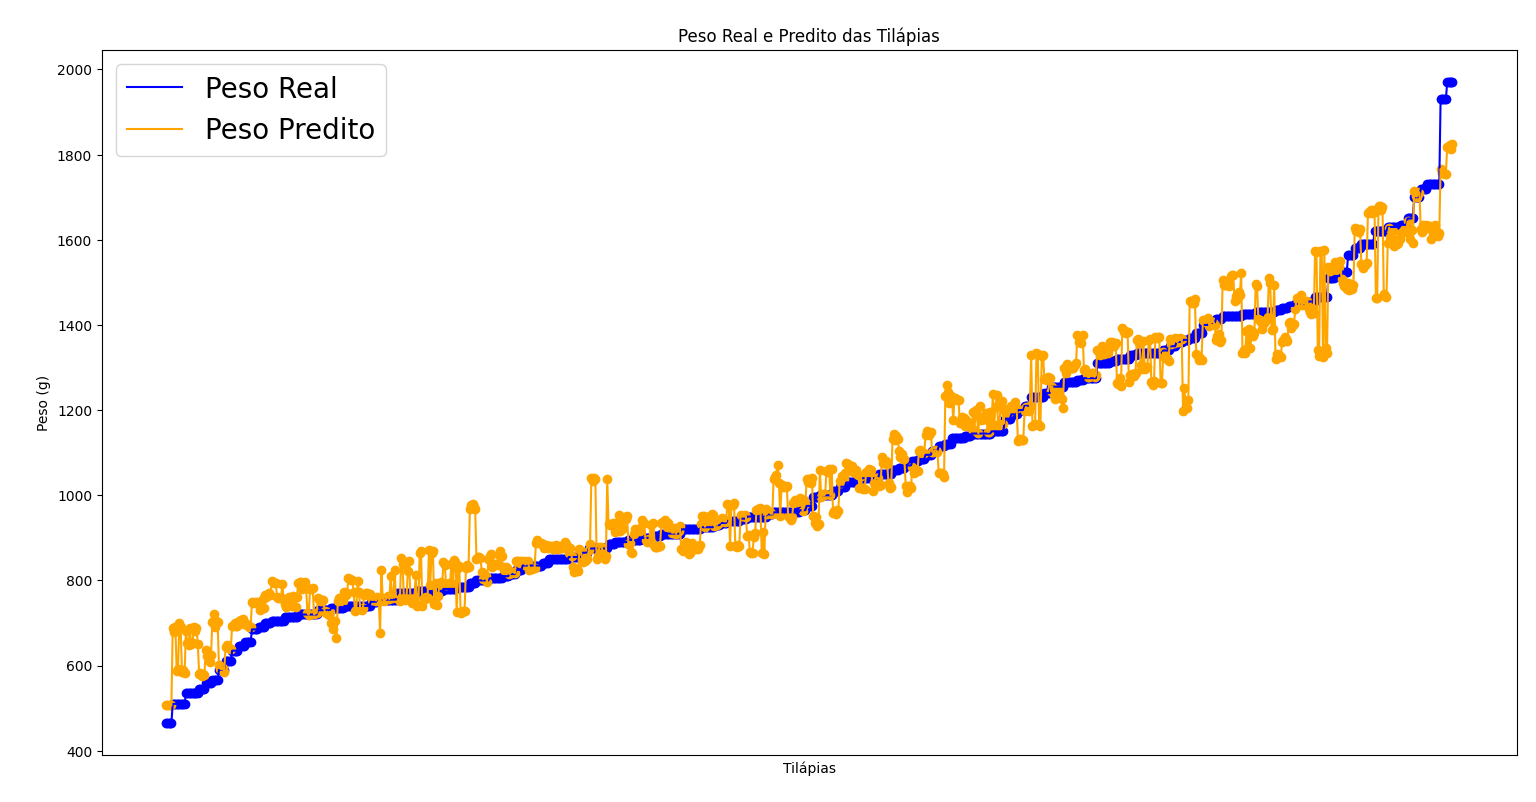
\includegraphics[width=\linewidth]{figura14.png}
\caption{Comparativo dos pesos reais (azul) e preditos (laranja) usando Nadam (30 épocas, 30 sementes, sem pré-processamento).}
\label{fig:grafico_resultado}
\Description{Gráfico de linha mostrando duas séries de dados (Peso Real e Peso Predito) muito próximas, indicando alta acurácia do modelo. O eixo Y varia de 400 g a 2000 g.}
\end{figure}

\subsection{Análise detalhada dos erros}
Uma análise complementar da distribuição dos erros absolutos mostrou que a maior parte das predições se concentra em uma faixa inferior a 60 g de diferença em relação ao peso real, com poucos \textit{outliers} acima de 100 g. Ao inspecionar qualitativamente tais casos, verificou-se que boa parte deles estava associada a imagens com reflexos muito intensos na pele do peixe, inclinações acentuadas ou enquadramento parcial do corpo, o que sugere que a CNN depende fortemente da integridade da silhueta para realizar estimativas mais precisas.

Considerando o conjunto de teste como um todo, a soma dos pesos reais foi de aproximadamente 1034{,}33 kg, enquanto a soma dos pesos preditos foi de 1045{,}92 kg, resultando em diferença global de cerca de -11{,}60 kg entre ambos. O desvio padrão dos erros absolutos foi da ordem de 38{,}09 g e o desvio padrão dos erros percentuais de 4{,}82\%. Esses valores indicam que, embora exista uma leve tendência à superestimação dos pesos, a maioria das predições permanece em uma faixa considerada aceitável para aplicações de campo, especialmente quando comparada às variações inerentes ao processo de pesagem manual.

Além disso, observou-se uma leve tendência de superestimação dos pesos em animais mais leves e subestimação em animais mais pesados, indicando uma possível regressão à média. Esse comportamento é comum em problemas de regressão e pode ser mitigado em trabalhos futuros com arquiteturas mais sofisticadas ou com a inclusão de informações biométricas adicionais, como o comprimento do peixe.

\subsection{Curvas de aprendizado e estabilidade dos otimizadores}
As curvas de aprendizado revelaram convergência relativamente rápida nas primeiras épocas, seguida por um \textit{plateau} nas etapas finais. Em algumas configurações sem \textit{Dropout}, sinais de \textit{overfitting} começaram a aparecer com o aumento do número de épocas, reforçando a importância do uso combinado de regularização L2 e \textit{Dropout} nas camadas densas.

Comparando Adam e Nadam, este último apresentou trajetórias de perda mais suaves e estabilidade superior em cenários com maior variabilidade luminosa, o que está em linha com a literatura sobre o uso de gradiente acelerado de Nesterov em superfícies de perda não convexas \cite{Ruder2016}. Em particular, o Nadam mostrou-se menos sensível a escolhas específicas de semente de inicialização, produzindo resultados mais consistentes entre diferentes execuções.

\subsection{Discussão}
O desempenho superior do Nadam sobre o Adam pode ser atribuído à sua combinação do Adam com o \textit{Nesterov Accelerated Gradient} (NAG) \cite{Ruder2016}. O Nadam antecipa a direção do gradiente, o que proporciona maior estabilidade em superfícies de perda ruidosas, como as geradas pela variabilidade de iluminação e posicionamento das tilápias nos dados de treino.

\textbf{Comparação com o manejo tradicional:} Quando comparado ao processo manual de pesagem por amostragem, que exige, no mínimo, dois operadores, equipamentos específicos e, em alguns casos, sedação, o modelo proposto oferece um ganho potencial em termos de segurança, tempo e bem-estar animal. Ainda que a solução atual exija a captura do peixe para obtenção da imagem, abre-se caminho para futuramente integrar o modelo a sistemas de captura automática de imagens, inclusive subaquáticas, reduzindo mais ainda a intervenção humana.

\textbf{Impacto na cadeia produtiva:} Em um cenário de produção intensiva, estimativas de peso mais frequentes permitem ajustes finos na taxa de arraçoamento e na densidade de estocagem, com impacto direto em custos de ração e sanidade. Um sistema baseado neste modelo poderia, por exemplo, ser acoplado a uma esteira de classificação ou a um módulo de triagem automática, fornecendo estimativas em tempo quase real para apoio à tomada de decisão.

\textbf{Limitações observadas:} Entre as principais limitações do trabalho destacam-se: (i) a ausência de variáveis físicas adicionais (como comprimento corporal) como entradas do modelo, (ii) a heterogeneidade das condições de iluminação e enquadramento das imagens, que prejudicou o pré-processamento, e (iii) o tamanho relativamente limitado da base em termos de diversidade de cenários de captura. Esses fatores indicam que, embora os resultados sejam encorajadores, ainda é necessário validar a abordagem em bancos de dados maiores, mais variados e coletados em diferentes ambientes de produção, de modo a descartar a possibilidade de um \textit{falso positivo} em termos de generalização.

% --------------------------------------------------------------
\section{Conclusão e Trabalhos Futuros}
% --------------------------------------------------------------
Este estudo demonstrou com sucesso o potencial das Redes Neurais Convolucionais para a predição de peso de tilápias a partir de imagens, alcançando um Erro Absoluto Médio (MAE) aceitável (45--50 g) e um Coeficiente de Determinação ($R^2$) superior a 0{,}90 na maioria dos casos. A análise detalhada dos erros mostrou que a maior parte das predições se mantém dentro de uma faixa estreita em torno dos valores reais, com desvio padrão dos erros absolutos em torno de 38 g e erro percentual médio inferior a 5\%, o que é compatível com aplicações práticas em piscicultura intensiva.

Identificamos limitações importantes: (1) a ausência de dados físicos complementares, como o comprimento do peixe, que poderiam melhorar a precisão; (2) a variabilidade na qualidade das imagens (iluminação, posicionamento); e (3) o fracasso do \textit{pipeline} de pré-processamento de imagens, que necessita de maior refinamento. Também foi observada uma leve tendência à superestimação dos pesos preditos, apontando para a necessidade de calibração adicional do modelo ou de técnicas de pós-processamento para correção de viés.

Como trabalhos futuros, sugerimos:
\begin{itemize}
    \item Investigar métodos menos invasivos de obtenção de imagem (ex.: câmeras subaquáticas), eliminando a necessidade de remover o peixe da água e aproximando o sistema de um cenário de monitoramento contínuo.
    \item Integrar outras variáveis de entrada no modelo (ex.: comprimento e largura do peixe) para uma predição multimodal, combinando informações morfométricas explícitas com características extraídas automaticamente pelas CNNs.
    \item Explorar arquiteturas mais avançadas, como Redes Residuais (ResNets) e modelos leves (MobileNet, EfficientNet), bem como técnicas de \textit{Transfer Learning}, de forma a avaliar o ganho de desempenho em comparação à arquitetura atual.
    \item Validar o modelo em bancos de dados maiores e mais diversificados, coletados em diferentes sistemas de produção e sob variadas condições de iluminação, para garantir a generalização e descartar a possibilidade de um falso positivo.
    \item Investigar o uso de módulos de segmentação ou detecção de pontos anatômicos, capazes de isolar o contorno corporal da tilápia, reduzindo a influência de reflexos e ruídos de fundo sobre as predições.
\end{itemize}

Além dessas perspectivas, a implementação de técnicas de \textit{Transfer Learning}, utilizando redes pré-treinadas em grandes bases de imagens naturais, surge como uma alternativa promissora para reduzir o tempo de treinamento e potencialmente melhorar a capacidade de generalização do modelo em cenários de poucos dados rotulados. Arquiteturas leves, como MobileNet ou EfficientNet, também se mostram interessantes para futura implantação em dispositivos embarcados, aproximando a solução proposta de aplicações em tempo real em unidades produtoras.

Do ponto de vista prático, recomenda-se, ainda, o avanço em diretrizes de captura de imagens em campo, como padronização de distância da câmera, controle básico de iluminação e manutenção de um fundo contrastante. Esses cuidados simples podem melhorar significativamente a qualidade das predições sem exigir modificações profundas na arquitetura da rede.

A automação desse processo tem potencial para melhorar significativamente o manejo na piscicultura, reduzindo custos, promovendo o bem-estar animal e aumentando a eficiência produtiva. Ao aproximar a tilapicultura de práticas de agricultura digital, este trabalho contribui com uma base experimental sólida sobre a qual soluções mais completas e integradas podem ser construídas nos próximos anos.

% --------------------------------------------------------------
%                 BIBLIOGRAFIA
% --------------------------------------------------------------
\bibliographystyle{ACM-Reference-Format}
\bibliography{referencias_tcc} % Nome do arquivo .bib

\end{document}
